%; whizzy chapter
% -initex iniptex -latex platex -format platex -bibtex jbibtex -fmt fmt
% $B0J>e(B whizzytex $B$r;HMQ$9$k>l9g$N@_Dj!#(B

%     Kansai Debian Meeting resources
%     Copyright (C) 2007 Takaya Yamashita
%     Thank you for Tokyo Debian Meeting resources

%     This program is free software; you can redistribute it and/or modify
%     it under the terms of the GNU General Public License as published by
%     the Free Software Foundation; either version 2 of the License, or
%     (at your option) any later version.

%     This program is distributed in the hope that it will be useful,
%     but WITHOUT ANY WARRANTY; without even the implied warranty of
%     MERCHANTABILITY or FITNESS FOR A PARTICULAR PURPOSE.  See the
%     GNU General Public License for more details.

%     You should have received a copy of the GNU General Public License
%     along with this program; if not, write to the Free Software
%     Foundation, Inc., 51 Franklin St, Fifth Floor, Boston, MA  02110-1301 USA

%  preview (shell-command (concat "evince " (replace-regexp-in-string "tex$" "pdf"(buffer-file-name)) "&"))
% $B2hA|%U%!%$%k$r=hM}$9$k$?$a$K$O(Bebb$B$rMxMQ$7$F(Bboundingbox$B$r:n@.!#(B
%(shell-command "cd image200708; ebb *.png")

%%$B$3$3$+$i%X%C%@3+;O!#(B

\documentclass[mingoth,a4paper]{jsarticle}
\usepackage{kansaimonthlyreport}
\usepackage[dvips]{xy}

% $BF|IU$rDj5A$9$k!"Kh7nJQ$o$j$^$9!#(B
\newcommand{\debmtgyear}{2010}
\newcommand{\debmtgdate}{24}
\newcommand{\debmtgmonth}{01}
\newcommand{\debmtgnumber}{31}

\begin{document}

\begin{titlepage}

% $BKh7nJQ99$9$kItJ,!"K\J8$NKvHx$b=$@5$9$k$3$H$r$o$9$l$:$K(B

 $BBh(B\debmtgnumber{}$B2s(B $B4X@>(B Debian $BJY6/2q;qNA(B

\vspace{2cm}

\begin{center}

\includegraphics{image200802/kansaidebianlogo.png}
\end{center}

\begin{flushright}
\hfill{}$B4X@>(B Debian $BJY6/2qC4Ev<T(B $B:4!9LZ!&ARI_!&$N$,$?(B \\
\hfill{}\debmtgyear{}$BG/(B\debmtgmonth{}$B7n(B\debmtgdate{}$BF|(B
\end{flushright}

\thispagestyle{empty}
\end{titlepage}

\dancersection{Introduction}{Debian JP}

\subsection*{}%$B%m%4MQ$N%9%Z!<%92T$.(B
 
$B4X@>(B Debian $BJY6/2q$O(BDebian GNU/Linux $B$N$5$^$6$^$J%H%T%C%/(B($B?7$7$$%Q%C%1!<(B
$B%8!"(BDebian $BFCM-$N5!G=$N;EAH!"(BDebian $B3&7($G5/$3$C$?=PMh;v!"$J$I$J$I!K$K(B
$B$D$$$FOC$79g$&2q$G$9!#(B

$BL\E*$H$7$F<!$N;0$D$r9M$($F$$$^$9!#(B
\begin{itemize}
      \item ML$B$d7G<(HD$G$O$J$/!"D>@\4i$r9g$o$;$k;v$G$N>pJs8r49$NB%?J(B
      \item $BDj4|E*$K=8$^$l$k>l=j(B
      \item $B;qNA$N:n@.(B
\end{itemize}

$B$=$l$G$O!"3Z$7$$0l;~$r$*3Z$7$_2<$5$$!#(B

\clearpage

\begin{minipage}[b]{0.2\hsize}
 {\rotatebox{90}{\fontsize{80}{80}
{\gt $B4X@>%G%S%"%sJY6/2q(B}}}
\end{minipage}
\begin{minipage}[b]{0.8\hsize}
\hrule
\vspace{2mm}
\hrule
\setcounter{tocdepth}{1}
\tableofcontents
\vspace{2mm}
\hrule
\end{minipage}

\dancersection{$B:G6a$N(BDebian$B4X78$N%$%Y%s%HJs9p(B}{Debian JP}

\subsection{$BA02s$N4X@>(B Debian $BJY6/2q(B}

$BA02s$N4X@>(B Debian $BJY6/2q$O(B 2009 $BG/(B 12 $B7n(B 27 $BF|$KBg:eJ!Eg6hL1%;%s%?!<$K(B
$B$F3+:E$5$l$^$7$?!#(B

$BH/I=$O!"(B
$B$^$5$5$s$K$h$k!"(B
GPS $B%l%7!<%P$H(B EeePC $B$rAH$_9g$o$;$F(B
$B<+J,$N8=:_CO$r%j%"%k%?%$%`$KI=<($5$;$k!V%O%s%I%a%$%I(B GPS $B%m%,!<$N9=C[!W$H!"(B
%
$B$?$J$+$H$7$R$5$5$s$K$h$k!"(B
Open Street Map $B$N>R2p$H(B Debian $B$G$N<B1i(B
$B!V(BDebian$B$r;H$C$FL{$7$`(B Open Street Map $BF~Lg!W$G$7$?!#(B

$B4X@>(B Debian $BJY6/2q$G$O!":G6a(B GPS $B%m%,!<$r;}$C$F$$$k?M$,A}$($F$$$k$o$1$G$9$,!"(B
$B:#8e$^$9$^$9A}$($=$&$J5$$,$7$^$9(B\footnote{%
$B$H$$$&$+!"$D$$$K:4!9LZ$b9XF~$7$F$7$^$$$^$7$?(B($B>P(B)}$B!#(B%

\subsection{$BBh(B 60 $B2sEl5~%(%j%"(B Debian$BJY6/2q(B - BSP 2010/Tokyo}

1 $B7n(B 23 $BF|(B($B:rF|(B), 
$BBh(B 60 $B2sEl5~%(%j%"(B Debian$BJY6/2q(B - BSP 2010/Tokyo $B$,3+:E$5$l$^$7$?!#(B
$B$3$N869F$r<9I.$7$F$$$k;~E@$G$OL$Mh$N=PMh;v$J$o$1$G$9$,!"(B
($B62$i$/(B)$B@9Bg$K(B Bug Squash $B$,9T$J$o$l$?;v$HA[A|$5$l$^$9!#(B

Debian $B$N<!4|0BDjHG!"%3!<%I%M!<%`(B Squeeze $B$N%j%j!<%9%U%j!<%:$O(B
2010$BG/(B 3 $B7n$,M=Dj$5$l$F$$$^$9!#(B
$B%P%0DY$7$@$1$G$O$J$/%I%-%e%a%s%H(B/po $B$NK]Lu$J$I$d$C$F$*$-$?$$;v$,$"$k?M$O(B
$BAa$a$K$d$C$D$1$F$7$^$$$^$7$g$&!#(B

$B8=:_$N(B RC $B%P%0$N>u67$O(B
\url{http://bugs.debian.org/release-critical/} $B$G3NG'$G$-$^$9!#(B

\clearpage
\dancersection{Xen$B$G:n$k<+Bp%5!<%P(B}{$B@n9>(B $B9@(B}

\subsection{$B$O$8$a$K(B}
$B6aG/!"(BCPU$B$N@-G=$,%Q%o%U%k$K$J$k$K$D$l$F!"9b2A$J%O!<%I%&%'%"$rA0Ds$H$7$?(B
$B2>A[2=5;=Q$,%Q!<%=%J%k%Y!<%9$G$b;H$($k$h$&$K$J$C$F$-$^$7$?!#(B

$B$=$3$G!"5S8w$rMa$S$F$-$?2>A[2=5;=Q$NBeI=3J$G$"$k(BXen$B$r;H$C$F!"%$%s%?%M%C(B
$B%H4XO"$N%5!<%P72$r9=C[$7$^$7$?$N$G!"(BDebian$B%Y!<%9$G(BXen$B$N2>A[%5!<%P$r9=C[(B
$B$9$k;~$KCm0U$9$k$3$H$d!">e5-%5!<%P72$r9=C[$9$k:]$K;W$C$?$3$H$r%l%]!<%H(B
$B$7$^$9!#(B

$B$^$?!"0J2<$N;EMM$O%Q!<%=%J%k%Y!<%9$G$N1?MQ$rA0Ds$K9=C[$7$?$b$N$G$9!#;E(B
$BMM$r;n$=$&$H$9$k$H$-$O!"I,$:%G!<%?Ey$N%P%C%/%"%C%W$r$H$C$F<+8J@UG$$G9T$C(B
$B$F$/$@$5$$!#$h$j>\$7$/CN$j$?$$J}$O@lLg=q$r;2>H$7$F$/$@$5$$!#(B

\subsection{Xen$B$H$O(B}
Xen$B$O!"2>A[%^%7%s%=%U%H%&%'%"$N0l$D$G!"(BOS$B$h$j(B1$B$D$N2<$N3,AX$G%O%$%Q!<%P(B
$B%$%6$H$$$&%W%m%0%i%`$rF0$+$9$b$N$G$9!#$3$N%?%$%W$O%O%$%Q!<%P%$%67?$H8F(B
$B$P$l!"!V(BVMware Infrastrucure$B!W$J$I$,$"$j$^$9!#(B

$BB>J}!"2>A[%^%7%s%=%U%H%&%'%"$K$O%"%W%j%1!<%7%g%s%?%$%W$H8F$P$l$k$b$N$,(B
$B$"$j!"!V(BVMware Workstation$B!W!V(BVirtualBox$B!W!V(BQEMU$B!W$,M-L>$G$9!#(B

\subsection{Xen$B$NFCD'(B}
Xen$B$O2>A[2=$9$k$?$a$N%b%G%k$H$7$F!"=`2>A[2=$H40A42>A[2=$N(B2$B$D$rDs6!$7$F$$$^$9!#(B
\begin{itemize}
\item $B=`2>A[2=(B(ParaVirtualization)\\
Xen$B$G$N=`2>A[2=$O%O!<%I%&%'%"$r%(%_%e%l!<%H$9$kBe$o$j$K!"2>A[%^%7%sMQ$N%O!<%I%&%'%"$r;HMQ$7$^$9!#$3$N%O!<%I%&%'%"$OA`:n$r$9$k$?$a$K%O%$%Q!<%P%$%6%3!<%k$r8F$S=P$7$^$9!#%O%$%Q!<%P%$%6%3!<%k$O2>A[%^%7%s4D6-$KBP1~$7!"(BOS$B$O(BXen$B2>A[%O!<%I%&%'%"MQ$K=$@5$9$kI,MW$,$"$j$^$9!#(B

\item $B40A42>A[2=(B(FullVirtualization)\\
Xen$B$O40A42>A[2=5!G=$bDs6!$7$F$$$^$9!#$3$N5!G=$rMxMQ$9$k$H!"%G%U%)%k%H$N(BOS$B$r$=$N$^$^(BXen$B>e$GF0:n$5$;$k$3$H$,$G$-$^$9!#(B
\end{itemize}

\subsection{Xen$B$N7ABV(B}
Xen$B$O(BLinux$B$r%Y!<%9$K:n$i$l$F$$$^$9$N$G!"(BXen$BMQ$K%3%s%Q%$%k$5$l$?%+!<%M%k$rMxMQ$7$^$9!#$3$N%+!<%M%k$O5/F0;~$K%O%$%Q!<%P%$%6$r%m!<%I$7!"$=$N>e$K%+!<%M%k$r%m!<%I$7$^$9!#%$%a!<%8E*$K$O%O%$%Q!<%P%$%6>e$r4IM}(BOS$B$N(BDomainO$B$,F0$-!"$=$N(BOS$B$K4IM}$5$l$k7A$G%2%9%H(BOS$B$H8F$P$l$k(BDomainU$B$,F0$-$^$9!#(B

\begin{itemize}
\item Domain-O $B!J4IM}(BOS$B!K0J2<(BDomO \\
      Xen$B$r5/F0$7$?(BOS$B!#%O!<%I%&%'%"$r4IM}$7!"%O%$%Q!<%P%$%6>e$GF0:n$9$k%2%9%H(BOS$B$N4IM}$r9T$&!#(B
\item Domain-U $B!J(BDomU-$B=`2>A[2=!K0J2<(BDomU \\
      Domain-O$B$K$h$C$F5/F0!"4IM}$5$l$k%2%9%H(BOS$B!#FC$K!"=`2>A[2=$GF0:n$9$k!#(B
\item HVM Domain $B!J(BHVM-$B40A42>A[2=!K0J2<(BHVM \\
      Domain-O$B$K$h$C$F5/F0!"4IM}$5$l$k%2%9%H(BOS$B$G$"$k$,!"40A42>A[2=$G$"$k(BHVM(Hardware Virtual Machine)$B$GF0:n$9$k!#(B
\end{itemize}

%$B?^7A$NA^F~(B
\begin{figure*}[h!]
 \centering
 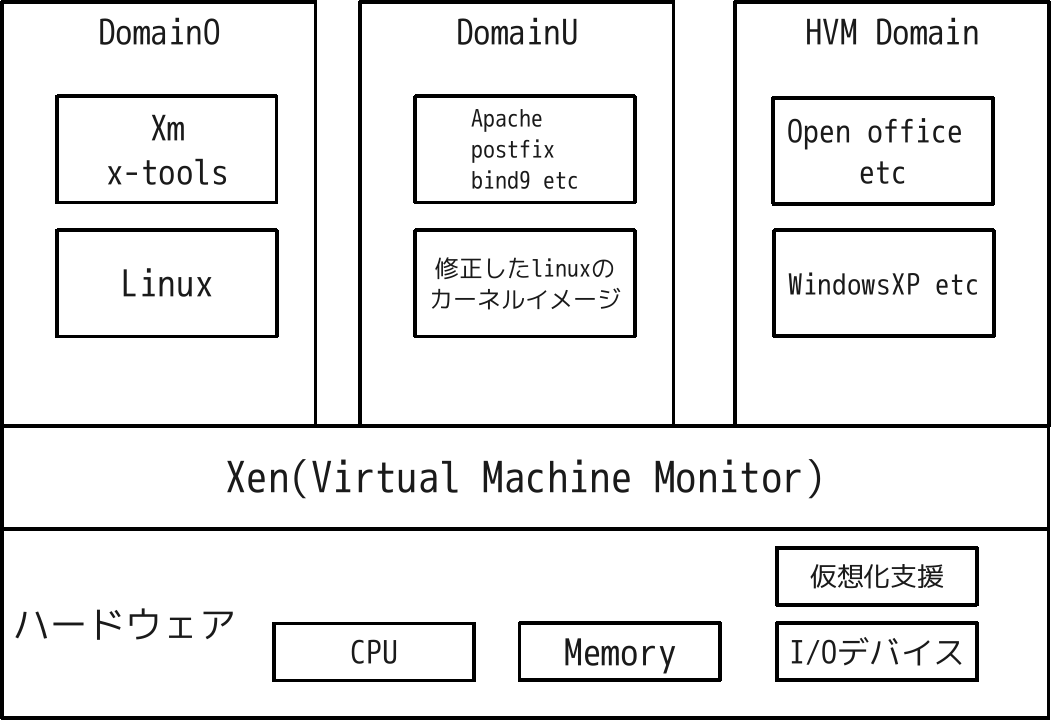
\includegraphics[scale=0.6]{image201001/xen-image.png}
 \caption{Xen $B$N%O%$%Q!<%P%$%6%b%G%k$N%$%a!<%8(B}
\end{figure*}
\clearpage

\subsection{Xen $B$NF3F~(B}
$B<!$K(B, Xen $B$r%$%s%9%H!<%k$7$^$9(B. $B%$%s%9%H!<%k$O3F%"!<%-%F%/%A%c$K$h$C$F0[$J$j$^$9(B. \footnote{$B>\$7$/$O(B, $B2>A[2=5;=Q(B Xen -$B35G0$HFbIt9=B$$J$I$r;2>H$7$F$/$@$5$$(B. $B40A42>A[2=$rL\E*$K$9$k$N$G$"$l$P(B Intel-VT $B$d(B AMV-V $B$,(B, CPU $B$G2>A[2=;Y1g5!G=$r;}$C$F$$$^$9(B. } $B$3$3$G$O(B, $B%$%s%F%k$r%Y!<%9$K(B Lenny $B$N(B Xen $B%+!<%M%k%$%a!<%8(B 2.6.26 $B$r0J2<$NMM$K%$%s%9%H!<%k$7$^$9(B.

\begin{commandline}
# aptitude install xen-linux-system-2.6.26-2-xen-686 
\end{commandline}
$B$^$?(B, Debian $B$K$O(B DomU $B$r:n$k%D!<%k$bMQ0U$7$F$"$j$^$9$N$G(B, $B$3$l$b%$%s%9%H!<%k$7$^$9(B.
\begin{commandline}
# aptitude install xen-tools
\end{commandline}
$B3F%$%s%9%H!<%k$,:Q$s$@$i(B, /xen/xen/xend-config.sxp $B%U%!%$%k$N0J2<$N2U=j$rJQ$($^$9(B.
\begin{commandline}
(network-script 'network-bridge netdev=eth1')
(network-script 'network-bridge netdev=eth0')
\end{commandline}
$B:F5/F0$7(B, DomO $B$N5/F0$r3NG'$7$^$9(B.
\begin{commandline}
# xm list
Name                 ID   Mem  VCPUs   State   Time (s)
Domain-0             0   1478     1   r-----    217.6
\end{commandline}

\subsection{DomU $B$N@_Dj(B}
Xen $B$N%D!<%k$r;H$C$F%2%9%H(B OS $B$r0J2<$N<j=g$GF~$l$^$9(B. (etch $B$d(B Ubuntu, CentOS $B$b2DG=(B).
\begin{enumerate}
\item $B@_Dj%U%!%$%k$NJT=8(B
\item xen-create-image $B$N<B9T(B
\item DomU $B$N5/F0(B
\end{enumerate}

\subsubsection{$B@_Dj%U%!%$%k$NJT=8(B}
$B@_Dj%U%!%$%k$O(B, /etc/xen-tools/xen-tools.conf $B$G$9(B. $B0J2<(B, DomU $B$K(B Lenny $B$r%$%s%9%H!<%k$b$N$H$7$FJT=8$7$^$9(B.

%$B2~%Z!<%8(B, $BCm0U(B
\begin{commandline}
##
#  /etc/xen-tools/xen-tools.conf
##             ($BCfN,(B)
#  Output directory for storing loopback images.
#
#  If you choose to use loopback images, which are simple to manage but
# slower than LVM partitions, then specify a directory here and uncomment
# the line.
#
#  New instances will be stored in subdirectories named after their
# hostnames.
# 
##
dir = /home/xen ($B%$%a!<%8%U%!%$%k$NJ]4I>l=j$G$9(B)
#              ($BCfN,(B)

##
#  Disk and Sizing options.
##
size   = 4Gb      # Disk image size.
#memory = 128Mb    # Memory size
memory = 384Mb    # Memory size
#swap   = 128Mb    # Swap size
swap   = 512Mb    # Swap size
# noswap = 1      # Don't use swap at all for the new system.
fs     = ext3     # use the EXT3 filesystem for the disk image.
#dist   = etch     # Default distribution to install.
dist   = lenny     # Default distribution to install.

#  Currently supported and tested distributions include:
#
# via Debootstrap:
#
#  Debian:
#   sid, sarge, etch, lenny.($BB>$N%G%#%9%H%j%S%e!<%7%g%s$NA*Br$b2DG=(B)
#
#  Ubuntu:
#   edgy, feisty, dapper.
#
# via Rinse:
#   centos-4, centos-5.
#   fedora-core-4, fedora-core-5, fedora-core-6, fedora-core-7

##
# Networking setup values.
##
#
## Uncomment and adjust these network settings if you wish to give your
# new instances static IP addresses.
#
# gateway   = 192.168.1.1
gateway   = 192.168.0.1
# netmask   = 255.255.255.0
netmask   = 255.255.255.0
# broadcast = 192.168.1.255
broadcast = 192.168.0.255
#($B%M%C%H%o!<%/$O$4<+M3$K(B)

#($B0J2<$O%G%U%)%k%H$K$7$^$7$?(B)
# Default kernel and ramdisk to use for the virtual servers
#
kernel      = /boot/vmlinuz-`uname -r`
initrd      = /boot/initrd.img-`uname -r`

#  The architecture to use when using debootstrap, rinse, or rpmstrap.
#
#  This is most useful on 64 bit host machines, for other systems it
# doesn't need to be used.
#
# arch=[i386|amd64]
#

# The default mirror for debootstrap to install Debian-derived distributions
#
mirror = http://ftp.jp.debian.org/debian/

#  If you're using the lenny or later version of the Xen guest kernel you will
# need to make sure that you use 'hvc0' for the guest serial device,
# and 'xvdX' instead of 'sdX' for serial devices.
#
#  You may specify the things to use here:
#
serial_device = hvc0 #default
# serial_device = tty1
#
disk_device = xvda #default
# disk_device = sda

#  Here we specify the output directory which the Xen configuration
# files will be written to, and the suffix to give them.
#
#  Historically xen-tools have created configuration files in /etc/xen,
# and given each file the name $hostname.cfg.  If you want to change
# that behaviour you may do so here.
#
# output    = /etc/xen
# extension = .cfg
#
\end{commandline}

\subsubsection{xen-create-image $B$N<B9T(B}
$B<!$K(B, DomU $B$N%$%a!<%8$r:n$j$^$9(B. $BF1;~$K(B DomU $B$K3d$jEv$F$k(B IP $B%"%I%l%9$r%*%W%7%g%s$G;XDj$7$^$9(B. $BNc$($P(B, $B%"%I%l%9$r(B 192.168.0.2, $B%[%9%H%M!<%`$r(B dns $B$H$9$k$J$i0J2<$N$h$&$K$7$^$9(B.
\begin{commandline}
# xen-create-image --ip 192.168.0.2 --hostname dns
\end{commandline}
DomU $B$N@):n$K$O(B, $B%$%a!<%8%G%#%9%/$NBg$-$5$d%M%C%H%o!<%/$N>u67$K$h$C$F0[$J$j$^$9$,(B, $B<+J,$N4D6-$G$O(B 10G $B$N%$%a!<%8$G(B 30 $BJ,$0$i$$$G$7$?(B.

\subsubsection{DomU $B$N5/F0(B}
$BL5;v$K(B, $B%$%s%9%H!<%k$,$G$-$?$i5/F0$7$F(B, $B2TF/>u67$r8+$F$_$^$7$g$&(B.
\footnote{Xen $B$K$O4IM}MQ%D!<%k$H$7$F!V(B xm $B!W$J$I$,$"$j$^$9(B. $B>\$7$/$O(B, Xen $BE0DlF~Lg$J$I$r;2>H$7$F$/$@$5$$(B. }
\begin{commandline}
# xen create -c dns.cfg
# xm list
 Name                                        ID   Mem VCPUs      State   Time (s)
 Domain-0                                     0  1478     4     r-----    429.8
 dns                                          5   384     1     -b----     10.5
 mail                                         2   384     1     -b----    123.6
 www                                          4  1792     1     -b----     23.1
\end{commandline}
$B5/F0$7$F$/$k2hLL$O(B, $BA4$/$N=i4|>uBV$G%m%0%$%s%W%m%s%W%H$7$+=P$^$;$s(B. root $B$G%m%0%$%s$7$F%Q%9%o!<%I$H%f!<%6$r:n@.$7$^$9(B.
\begin{commandline}
# passwd
# adduser ipv6waterstar
\end{commandline}
\subsubsection{$B%P%C%/%"%C%W(B, $BB>(B}
$B$^$?(B, DomU $B$r%G%U%)%k%H$G%$%s%9%H!<%k$7$?>l9g(B, DomO $B$N(B/home/xen/domain $B$K3F(B DomU $B$N%I%a%$%s$4$H$K%a!<%8%U%!%$%k$,CV$+$l$^$9(B. $B$^$?(B, $B@_Dj%U%!%$%k$O(B/etc/xen $B$K(B  ".cfg"$B%U%!%$%k$H$7$FJ]B8$5$l$^$9(B.

$B=>$C$F(B, $BNc$($P2?$i$+$N@_Dj%_%9$r$7$F(B DomU $B$,5/F0ITG=$K$J$C$F$b(B, $B>e5-$N%$%a!<%8$H@_Dj%U%!%$%k$N%P%C%/%"%C%W$,$"$l$P(B, $B3F%G%#%l%/%H%j$H@_Dj%U%!%$%k$r$=$N$^$^%3%T!<$7D>$9$@$1$G(B, $BF1$84D6-$N(B DomU $B$rI|85$G$-$^$9(B.

$B$^$?(B, $B4IM}MQ$N(B DomO $B$O%;%-%e%j%F%#$N4X78$+$i%W%m%;%9?t$,>/$J$$J}$,$$$$$N$G$9$,(B, $B8e=R$N$h$&$K@_Dj%U%!%$%k$rB??t(B, $B:n@.$9$k>l9g$N$3$H$b9M$($k$H(B, GUI $B$GA`:n$,$G$-$k$J$I$NMxE@$+$i(B, gnome $B$J$I$r%$%s%9%H!<%k$9$k$3$H$r4+$a$^$9(B.


\subsection{Xen $B$N%M%C%H%o!<%/$N35MW(B}
Xen $B$O2>A[%$%s%?!<%U%'%$%9$r%Y!<%9$K$7$?%M%C%H%o!<%/5!G=$r;}$C$F$$$^$9(B.

$B6qBNE*$K$O(B, DomU $B$N3F%[%9%H$rD>@\30It%M%C%H%o!<%/$K@\B3$9$k%V%j%C%87PM3$N@\B3(B. $B2>A[%$%s%?!<%U%'%$%9$rDL$7$F(B, DomO $B$N%k!<%F%#%s%0$7(B, $B%M%C%H%o!<%/%$%s%?!<%U%'%$%9$K=PNO$9$k%V%j%C%8$r7PM3$7$J$$@\B3(B (NAT $B@\B3(B) $B$NFs$D$N7ABV$,$"$j$^$9(B.

$B%V%j%C%87PM3$N@\B3$N%$%a!<%8$O%O!<%I%&%'%">e$K(B, DomO $B$HJ#?t$N(B DomU $B$N2>A[(B PC $B$,$"$C$F(B, $B$=$l$>$l$,BPEy$K%M%C%H%o!<%/%O%V$G7R$,$C$F$$$k$h$&$J>uBV$G$9(B.

$B:#2s$O(B, $B3F(B DomU $B%5!<%P$r%$%s%?!<%M%C%H%5!<%P$H$7$F1?MQ$7$?$$$N$G(B, $B2>A[%$%s%?!<%U%'%$%9$r;H$C$FD>@\(B, $B%;%0%a%s%H$,0[$J$k30It%M%C%H%o!<%/$K@\B3$G$-$k%V%j%C%87PM3$N@\B3$G%M%C%H%o!<%/$r9=@.$7$^$9(B.

DomU $B$O2>A[%^%7%s$r:n@.$9$k$H$-$K(B, IP $B%"%I%l%9$r3d$jEv$F$?$N$GFCJL$J@_Dj$OI,MW$"$j$^$;$s(B. $BF1;~$K(B, Mac $B%"%I%l%9$b3F2>A[%$%s%?!<%U%'%$%9$4$H$K<+F0E*$K3d$jEv$F$i$l$^$9(B.

$B$^$?(B, IP $B%"%I%l%9$r8e$+$iJQ99$7$?$$$H$-$J$I$O(B/etx/xen $B0J2<$N(B".cfg"$B%U%!%$%k$r=q$-49$($^$9(B.

$BNc(B  dns.cfg
%$B2~%Z!<%8(B  $BCm0U(B
\begin{commandline}
#
# Configuration file for the Xen instance www, created
# by xen-tools 3.9 on Tue Nov 17 10:35:03 2009.
#

#
#  Kernel + memory size
#
kernel      = '/boot/vmlinuz-2.6.26-2-xen-686'
ramdisk     = '/boot/initrd.img-2.6.26-2-xen-686'
memory      = '384'($B%a%b%j!<$NMFNL$NJQ99$b2DG=(B)

#
#  Disk device (s).
#
root        = '/dev/xvda2 ro'
disk        = [
                  'file:/home/xen/domains/www/swap.img,xvda1,w',
                  'file:/home/xen/domains/www/disk.img,xvda2,w',
              ]


#
#  Hostname
#
name        = 'dns'($B%[%9%HL>(B)

#
#  Networking
#
vif         = [ 'ip=192.168.0.2,mac=00:12:34:56:78:9A' ]
($B%"%I%l%9$NJQ99$b2DG=$G$9$,(B, DomU $B$N(B interfaces $B$r=q$-49$($F$$$k$H$-$O$=$A$i$b=q$-49$($F$/$@$5$$(B)

#
#  Behaviour
#
on_poweroff = 'destroy'
on_reboot   = 'restart'
on_crash    = 'restart'
\end{commandline}

\subsubsection{$B3F%$%s%?!<%M%C%H%5!<%P$N@_Dj$9$kA0$NCm0U;v9`(B}
$B<!$K(B, DNS, Mail $B%5!<%P(B, Web $B%5!<%P$N%Q%C%1!<%8$r(B, $B3F(B DomU $B$K%$%s%9%H!<%k$7$^$9(B.

$B%$%s%9%H!<%k$O(B, $B2>A[%^%7%s$G$b%N!<%^%k$N%$%s%9%H!<%k$HJQ$o$j$^$;$s(B. $B$?$@(B, Xen $B$N%M%C%H%o!<%/9=@.$OFHFC$N!VJJ!W$N$h$&$J$b$N$,$"$j$^$9(B. $B0J2<(B, $B$$$/$D$+Nc$r5s$2$^$9(B.
\begin{enumerate}
\item NTP $B$r;H$C$?;~4V$N@_Dj(B 
\item SSH $B$G$N%m%0%$%s(B
\item $B$=$NB>(B 
\end{enumerate}

\subsubsection{NTP $B$r;H$C$?;~4V$N@_Dj(B}
DomU $B$O(B Dom0 $B$+$i$N$_;~9o$r99?7$G$-$k$H$$$&(B Xen $B$N;EMM$J$N$G(B, Dom0 $B$G;~9o$r9g$o$;$F$$$l$P(B, DomU $B$b@53N$J;~9o$rF@$k$3$H$,$G$-$^$9(B. $B$?$@(B, DomU $B$G(B ntpd $B$d(B ntpdate $B$r<B9T$9$k$N$G$"$l$P(B, $B;~9oF14|$G$-$J$$$3$H$,$"$j$^$9(B.

$BIaDL$K(B DomU $B$G;~7W$r9g$o$;$k$N$G$"$l$P(B, Aisa/Tokyo $B$K9g$o$;$k$3$H$GF|K\;~4V$K$G$-$^$9(B ($B%G%U%)%k%H$G$O(B UTC).
\begin{commandline}
# dpkg-reconfigure tzdata
# date
  Tue Jan 24 15:00:00 JST 2010
\end{commandline}

$B$^$?(B, DomU $B$G(B NTP $BEy$r;H$&$N$G$"$l$P(B, DomU $B$N(B/etc/sysctl.conf $B$K(B{\tt xen.independent\_wallclock=1}$B$r2C$($F:F5/F0$7$F$/$@$5$$(B.

\subsubsection{SSH $B$G$N%m%0%$%s(B}
Xen $B$G(B SSH $B$r;H$C$F(B, $B%M%C%H%o!<%/1[$7$K%m%0%$%s$9$k>l9g$bDL>o$HF1$8$G$,(B, $B%$%s%9%H!<%k$7$?$P$+$j$N(B DomU $B$O2?$bF~$C$F$$$J$$$N$G(B, $B$=$N$^$^$G$O%(%i!<$K$J$j$^$9(B.

$B6qBNE*$K$O(B, $B$^$:(B DomU $B$K(B SSH $B$r%$%s%9%H!<%k$7$^$9(B ($B%]!<%HHV9f$NJQ99$J$I$O$*9%$_$G(B).
\begin{commandline}
# aptitude install ssh
\end{commandline}

$B<!$K%m!<%+%k$+$i(B SSH $B$r;H$C$F%m%0%$%s$7$h$&$H$7$F$b(B, $B0J2<$N%(%i!<$,$G$^$9(B.
\begin{commandline}
$ ssh mail.kinsen.gr.jp
  ipv6waterstar@dns.kinsen.gr.jp's password: 
  PTY allocation request failed on channel 0
\end{commandline}

$B860x$O(B, xen-tools $B$r;H$C$?(B DomU $B$N9=C[$G!V(B udev $B$r%$%s%9%H!<%k$7$J$$$?$a!W$K5/$3$j$^$9(B. $B=>$C$F(B, DomU $B$K(B udev $B$r%$%s%9%H!<%k$9$k$3$H$G2r7h$7$^$9(B.
\begin{commandline}
# aptitude install udev
\end{commandline}

\subsubsection{$B$=$NB>(B}
$B$=$NB>(B, Xen $B$G%5!<%P$r1?MQ$9$k$H$-$K$$$/$D$+5$$E$$$?$b$N$r5s$2$^$9(B.

$B$^$:(B, DomO $B$H(B DomU $B$,%V%j%C%87PM3$G@\B3$7$F$$$k>l9g(B, iptables $B$G(B FORWARD $B$r;H$&$H(B DomU $B$+$i%M%C%H%o!<%/$K7R$,$i$J$$8=>]$,5/$3$j$^$9(B ($BM}M3$OITL@(B).

$B$^$?(B, $B40A42>A[2=$G%2%9%H(B OS $B$rF0$+$=$&$H$9$k$N$G$"$l$P(B, CD $B$r%2%9%H(B OS $B$+$i%^%&%s%H$7(B, VNC $B$J$I$rN)$A>e$2$F%$%s%9%H!<%k$9$kI,MW$,$"$j$^$9(B ($B8!>Z$O$7$F$^$;$s$N$G(B, $B2DG=$+$I$&$+$OITL@(B).

$B>\$7$/$O(B, $B0J2<$N%I%-%e%a%s%HEy$r;2>H$7$F$/$@$5$$(B.
\begin{itemize}
\item \url{http://wiki.debian.org/Xen}
\end{itemize}

\subsection{$B3F%$%s%?!<%M%C%H%5!<%P$N@_Dj(B}
$B<!$K(B, $B3F%$%s%?!<%M%C%H%5!<%P$N@_Dj$N<j=g$r@bL@$7$^$9(B. $B$3$3$G$N4D6-$O(B, $B%0%m!<%P%k(B IP $B%"%I%l%9$,(B 1 $B$D$G(B, $B%$%s%?!<%M%C%H$K$OEEOC2q<R$+$iDs6!$5$l$F$$$k%k!<%?$G30It%M%C%H%o!<%/$K(B, $B7R$,$C$F$$$k$3$H$rA0Ds$H$7$^$9(B.

\subsubsection{DNS $B$N35MW(B}
DNS $B%5!<%P$O%[%9%HL>$H(B IP $B%"%I%l%9$rBP1~$5$;$?%>!<%s$H8F$P$l$k%U%!%$%k$r;}$A(B, $B%[%9%HL>$N8!:w$KBP$7$FBP1~$9$k(B IP $B%"%I%l%9$rJV$7$^$9(B. $B$^$?(B, $B%>!<%s%U%!%$%k$NFbMF$rB>$N%5!<%P$KE>Aw$7$^$9(B.

$B6qBNE*$K(B www.kinsen.gr.jp $B$H$$$&%[%9%HL>$KBP1~$9$k(B IP $B%"%I%l%9$r(B ($B:F5"(B) $B8!:w$9$k>l9g(B, $B$^$:(B, jp $B%I%a%$%s$N(B IP $B%"%I%l%9$rLd$$9g$o$;$kI,MW$,$"$j$^$9(B. $B$=$N$?$a$K(B, $B%k!<%H%5!<%P$G(B jp $B%I%a%$%s$N(B IP $B%"%I%l%9$r8!:w$7(B, jp $B%5!<%P$K@\B3$7$^$9(B. $BF1MM$K(B, jp $B$KB0$9$k(B gr $B%I%a%$%s$N(B IP $B%"%I%l%9$r8!:w$7(B, $B$5$i$K$O(B gr $B%I%a%$%s$KB0$9$k(B kinsen $B$=$7$F(B www $B$H=g<!(B, $B3F(B IP $B%"%I%l%9$r8!:w$7(B, $B3F%5!<%P$K@\B3$7$F$$$-$^$9(B. $B$=$7$F:G=*E*$K(B, www.kinsen.gr.jp $B$N(B IP $B%"%I%l%9$,(B 203.141.158.41 $B$G$"$k;v$,$o$+$j$^$9(B.

Debian $B$K$O(B DNS $B%5!<%P$H$7$F(B bind9 $B$N%Q%C%1!<%8$,MQ0U$5$l$F$$$^$9(B. $B0J2<(B, $B%$%s%9%H!<%k$H@_Dj$r9T$$$^$9(B.

\subsubsection{DNS $B$N@_Dj(B}
bind9, bind9utils $B%Q%C%1!<%8$r%$%s%9%H!<%k$7$^$9(B.
\begin{commandline}
# aptitude install bind9
# aptitude install bind9utils
\end{commandline}
$B:#2s$O%Q!<%=%J%k%f!<%9$J$N$G(B 1 $B8D$N%0%m!<%P%k(B IP $B%"%I%l%9$r;H$&$3$H$rA0Ds$H$7(B, $B%M!<%`%5!<%P$N@_Dj$K$O(B view $B$d(B match-client $B$r;H$$$^$9(B ($BNc$H$7$F(B, $BFbIt%>!<%s$G(B, 192.168.0.0/24 $B%M%C%H%o!<%/Fb$K3F%5!<%P$r(B, $B%0%m!<%P%k%"%I%l%9$H$7$F(B 203.141.158.41 $B$r;H$&$b$N$H$7$^$9(B).

view $B$O;XDj$N(B IP $B%"%I%l%9$d%M%C%H%o!<%/$4$H$K(B, $B8DJL$N%*%W%7%g%s$H%>!<%s%G!<%?$rDs6!$7$^$9(B.

$B6qBNE*$K$O(B, acl $B$G(B IP $B%"%I%l%9$H%M%C%H%o!<%/$r;XDj$7(B, match-clients $B$G(B acl $B$K%^%C%A$9$k%/%i%$%"%s%H$H(B, $B$=$NB>$N%/%i%$%"%s%H$4$H$KJL!9%>!<%s$rDs6!$7$^$9(B. $B$3$l$rMxMQ$7(B, 1 $BBf$N%5!<%P$GFbItMQ(B (acl $B$K%^%C%A$9$k(B) $B$H30ItMQ(B (acl $B$K%^%C%A$7$J$$(B) $B$N(B DNS $B$r9=C[$7$^$9(B.

$B$J$*(B, $B%0%m!<%P%k(B IP $B%"%I%l%9$,J#?t$N>l9g$O(B, $B3F(B DomU $B$K%0%m!<%P%k(B IP $B%"%I%l%9$r@_Dj$7$F$/$@$5$$(B. \footnote{$B>\$7$/$O(B, DNS BIND $BBh(B 5 $BHG$J$I$r;2>H$7$F$/$@$5$$(B. }

\subsubsection{view $B$N@_Dj(B}
$BDL>o(B, BIND $B$G(B view $B$r@_Dj$9$k>l9g(B, named.conf $B$K(B view $B$d(B acl, match-clients $B$N@_Dj$r=q$-2C$($^$9(B. $B$@$@(B, Debian $B$G$O(B, named.conf.options $B$d(B named.conf.local $B$J$I$N%U%!%$%k$,$"$j$^$9$N$G(B, $B$=$l$i$rMxMQ$7$^$9(B.

$B$^$:(B, named.conf $B$K0J2<$N$h$&$K=q$-49$((B, include $B$r;H$C$F@_Dj%U%!%$%k$rA^F~$9$k$h$&$K$7$^$9(B.
\begin{commandline}
// This is the primary configuration file for the BIND DNS server named.
//
// Please read /usr/share/doc/bind9/README.Debian.gz for information on the 
// structure of BIND configuration files in Debian, *BEFORE* you customize 
// this configuration file.
//
// If you are just adding zones, please do that in /etc/bind/named.conf.local
include "/etc/bind/named.conf.acl";  //view $B$r;H$&%"%I%l%9$NHO0O$r@_Dj$9$k(B
include "/etc/bind/named.conf.options";  //BIND $B$ND4@0$?$a$N%*%W%7%g%s(B
view "internal"{  // $BFbItMQ%>!<%s$N@_Dj(B
	match-clients { localnet; };  // $BFbIt%>!<%s$NE,MQHO0O$N@_Dj(B
	recursion yes;
include "/etc/bind/named.conf.conf";  // $BFbItMQ%>!<%s$N=i4|@_Dj(B
include "/etc/bind/named.conf.local";  // $BFbItMQ%>!<%s$N%m!<%+%k@_Dj(B
};
view "external" {  // $B30ItMQ%>!<%s$N@_Dj(B
	match-clients { any; };  // $B30It%>!<%s$NE,MQHO0O$N@_Dj(B
	recursion no;
include "/etc/bind/named.conf.view"; // $B30ItMQ%>!<%s$N%m!<%+%k@_Dj(B
};
\end{commandline}

\subsubsection{named.conf.acl $B$N@_Dj(B}
acl $B%9%F!<%H%a%s%H$G$O(B, $B%"%I%l%9%^%C%A%j%9%H$r@_Dj$7$^$9(B.

named.conf.acl $B$NFbMF$O0J2<$NDL$j(B
\begin{commandline}
acl localnet{ 
	192.168.0.0/24; 
	127.0.0.1; 
};
\end{commandline}

\subsubsection{named.conf.options $B$N@_Dj(B}
options $B%9%F!<%H%a%s%H$G$O(B, BIND $B$NF0:n$K4X$o$k$b$m$b$m$N%*%W%7%g%s$r@_Dj$7$^$9(B.

named.conf.options $B$NFbMF$O0J2<$NDL$j(B
\begin{commandline}
options {
	directory "/var/cache/bind";

	// If there is a firewall between you and nameservers you want
	// to talk to, you may need to fix the firewall to allow multiple
	// ports to talk.  See http://www.kb.cert.org/vuls/id/800113

	// If your ISP provided one or more IP addresses for stable 
	// nameservers, you probably want to use them as forwarders.  
	// Uncomment the following block, and insert the addresses replacing 
	// the all-0's placeholder.

	forwarders {
		123.456.789.001; 123.456.789.002;
            //ISP $B$G;XDj$5$l$?(B DNS $B$KBeM}Ld$$9g$o$;$rMW5a$9$k%"%I%l%9$r5-F~$7$^$9(B.
	 };

	allow-query { any; };  // $BLd$$9g$o$;2DG=$J%[%9%H$rL5@)8B$K(B
	allow-transfer { localnet; };  // $BE>Aw@h$r8BDj(B
	version "no version";  // $B%P!<%8%g%sI=<($rL58z$K(B
	auth-nxdomain no;    # conform to RFC1035
	listen-on-v6 { any; };

};
\end{commandline}

\subsubsection{named.conf.conf $B$N@_Dj(B}
$B$3$N%U%!%$%k$O$b$H$N(B named.conf ($B=i4|@_Dj(B) $B%U%!%$%k$G$9(B.

named.conf.conf $B$NFbMF$O0J2<$NDL$j(B.
\begin{commandline}
// prime the server with knowledge of the root servers
zone "." {
	type hint;
	file "/etc/bind/db.root";
};

// be authoritative for the localhost forward and reverse zones, and for
// broadcast zones as per RFC 1912

zone "localhost" {
	type master;
	file "/etc/bind/db.local";
};

zone "127.in-addr.arpa" {
	type master;
	file "/etc/bind/db.127";
};

zone "0.in-addr.arpa" {
	type master;
	file "/etc/bind/db.0";
};

zone "255.in-addr.arpa" {
	type master;
	file "/etc/bind/db.255";
};
\end{commandline}

\subsubsection{named.conf.local $B$N@_Dj(B}
$B%m!<%+%k%M%C%HMQ$N=i4|@_Dj%U%!%$%k(B.

named.conf.local $B$NFbMF$O0J2<$NDL$j(B
\begin{commandline}
//
// Do any local configuration here
//
zone "kinsen.gr.jp" {
	type master;
	file "/etc/bind/db.in-kinsen.gr.jp"; // $BFbIt=g0z$-%>!<%s%F!<%V%k(B
};
zone "0.168.192.in-addr.arpa" {
	type master;
	file "/etc/bind/db.192.168.0"; // $BFbIt5U0z$-%>!<%s%F!<%V%k(B
};
// Consider adding the 1918 zones here, if they are not used in your
// organization
//include "/etc/bind/zones.rfc1918";
\end{commandline}

$B0J2<$O3F%>!<%s%U%!%$%k$N@_DjNc$G$9(B.
\begin{enumerate}
\item $B=g0z$-%>!<%s%F!<%V%k(B
\begin{commandline}
;
; BIND data file for kinsen.gr.jp
;
$TTL	86400
@	IN	SOA	dns.kinsen.gr.jp. root.dns.kinsen.gr.jp. (
		              1		; Serial
			   1800		; Refresh
			    900		; Retry
			 604800		; Expire
			   1200 )	; Negative Cache TTL

                IN      NS      dns

; localhost
localhost       IN      A       127.0.0.1
localhost       IN      AAAA   ::1

; Mail exchange
                IN      MX   0  mail.kinsen.gr.jp.
;
; Host entry
;
noren           IN      A       192.168.0.1
;               IN      AAAA    2001:
dns             IN      A       192.168.0.2
;               IN      AAAA    2001:
mail            IN      A       192.168.0.3
;               IN      AAAA    2001:
www             IN      A       192.168.0.4
;               IN      AAAA    2001:
;
; Alias
;
;www            IN      CNAME   noren
;
; Domain
@               IN      A       192.168.0.2
                IN      MX 0    mail
\end{commandline}
\item $B5U0z$-%>!<%s%F!<%V%k(B
\begin{commandline}      
;
;BIND data file for 219.117.222 network
;
$TTL    86400
@       IN      SOA     dns.kinsen.gr.jp. root.dns.kinsen.gr.jp. (
                              1         ; Serial
                           1800         ; Refresh
                            900         ; Retry
                         604800         ; Expire
                           1200 )       ; Negative Cache TTL

                IN      NS      dns
;
; Host entry
;
1		IN      PTR     noren.kinsen.gr.jp.
2		IN      PTR     dns.kinsen.gr.jp.
3		IN      PTR     mail.kinsen.gr.jp.
4		IN      PTR     www.kinsen.gr.jp.
\end{commandline}
\end{enumerate}

\subsubsection{named.conf.view $B$N@_Dj(B}
$B%0%m!<%P%k%M%C%HMQ$N=i4|@_Dj%U%!%$%k$G$9(B.
named.conf.view $B$N@_Dj$O0J2<$NDL$j(B
\begin{commandline}   
zone "." {
	type hint;
	file "/etc/bind/db.root";
};
zone "kinsen.gr.jp"{
	type master;
	file "/etc/bind/db.out-kinsen.gr.jp"; // $B30It=g0z$-%>!<%s%F!<%V%k(B
	allow-transfer{ 
		localnet; 
		123.456.789.001; 
		123.456.789.002; 
	};
};
zone "158.141.203.in-addr.arpa"{
	type master;
	file "/etc/bind/db.203.141.158"; // $B30It5U0z$-%>!<%s%F!<%V%k(B
	allow-transfer{ 
		localnet;
		123.456.789.001;
		123.456.789.002; 
	};
};
\end{commandline}
$B0J2<$O3F%>!<%s%F!<%V%k$N@_DjNc$G$9(B.
\begin{enumerate}
\item $B=g0z$-%>!<%s%F!<%V%k(B
\begin{commandline}
;
; BIND data file for kinsen.gr.jp
;
$TTL	86400
@	IN	SOA	dns.kinsen.gr.jp. root.dns.kinsen.gr.jp. (
		              1		; Serial
			   1800		; Refresh
			    900		; Retry
			 604800		; Expire
			   1200 )	; Negative Cache TTL

		IN	NS	dns

; localhost
localhost       IN      A       127.0.0.1
localhost       IN      AAAA    ::1

; Mail exchange
        	IN      MX   0 mail.kinsen.gr.jp.
;
; Host entry
;
noren           IN      A      203.141.158.41
;               IN      AAAA   2001:
dns             IN      A      203.141.158.41
;               IN      AAAA   2001:
mail            IN      A      203.141.158.41
;               IN      AAAA   2001:
www             IN      A      203.141.158.41
;               IN      AAAA   2001:
;
; Domain
@               IN      A       203.141.158.41
                IN      MX 0    mail
\end{commandline}
\item $B5U0z$-%>!<%s%F!<%V%k(B
\begin{commandline}
;
;BIND data file for 203.141.158 network
;
$TTL    86400
@       IN      SOA     dns.kinsen.gr.jp. root.dns.kinsen.gr.jp. (
                              1         ; Serial
                           1800         ; Refresh
                            900         ; Retry
                         604800         ; Expire
                           1200 )       ; Negative Cache TTL

                IN      NS      dns
;
; Host entry
;
41		IN      PTR     noren.kinsen.gr.jp.
41		IN      PTR     dns.kinsen.gr.jp.
41		IN      PTR     mail.kinsen.gr.jp.
41		IN      PTR     www.kinsen.gr.jp.
\end{commandline}
\end{enumerate}
$B0J>e$N@_Dj$,=*$o$C$?$i(B, BIND $B$r:FFI$_9~$_(B, $B:F5/F0$7$^$9(B.
\begin{commandline}
# /etc/init.d/bind9 reload      $BCm!<I,$::FFI$_9~$_$+$i$7$F$/$@$5$$(B.
# /etc/init.d/bind9 restart  $B:FFI$_9~$_$G%(%i!<$,$G$?$iI,$:=$@5$7$F$/$@$5$$(B.
\end{commandline}
\clearpage

$B@5>o$KFI$_9~$_$,=*$o$C$?$i@_DjFbMF$r(B dig $B$d(B nslookup $B$r;H$C$F3N$+$a$^$9(B.
\begin{commandline}
$ dig @localhost dns.kinsen.gr.jp ($B%[%9%HL>$O$$$m$$$m;n$7$F$/$@$5$$(B)
; <<>> DiG 9.5.1-P3 <<>> @localhost dns.kinsen.gr.jp
; (2 servers found)
;; global options:  printcmd
;; Got answer:
;; ->>HEADER<<- opcode: QUERY, status: NOERROR, id: 55957
;; flags: qr aa rd ra; QUERY: 1, ANSWER: 1, AUTHORITY: 1, ADDITIONAL: 0

;; QUESTION SECTION:
;dns.kinsen.gr.jp.              IN      A

;; ANSWER SECTION:
dns.kinsen.gr.jp.     86400     IN      A       192.168.0.2

;; AUTHORITY SECTION:
kinsen.gr.jp.         86400     IN      NS      dns.kinsen.gr.jp.

;; Query time: 0 msec
;; SERVER: 127.0.0.1#53 (127.0.0.1)
;; WHEN: Thu Jan 21 07:26:57 2010
;; MSG SIZE  rcvd: 64

$ dig @localhost kinsen.gr.jp MX ($B%a!<%k$K$D$$$F$b3NG'$7$^$9(B)
; <<>> DiG 9.5.1-P3 <<>> @localhost kinsen.gr.jp MX
; (2 servers found)
;; global options:  printcmd
;; Got answer:
;; ->>HEADER<<- opcode: QUERY, status: NOERROR, id: 640
;; flags: qr aa rd ra; QUERY: 1, ANSWER: 1, AUTHORITY: 1, ADDITIONAL: 2

;; QUESTION SECTION:
;kinsen.gr.jp.                  IN      MX

;; ANSWER SECTION:
kinsen.gr.jp.           86400   IN      MX      0 mail.kinsen.gr.jp.

;; AUTHORITY SECTION:
kinsen.gr.jp.           86400   IN      NS      dns.kinsen.gr.jp.

;; ADDITIONAL SECTION:
mail.kinsen.gr.jp.      86400   IN      A       192.168.0.3
dns.kinsen.gr.jp.       86400   IN      A       192.168.0.2

;; Query time: 0 msec
;; SERVER: 127.0.0.1#53 (127.0.0.1)
;; WHEN: Thu Jan 21 07:25:15 2010
;; MSG SIZE  rcvd: 101

$ nslookup -type=mx kinsen.gr.jp ($B$3$N%3%^%s%I$G$b$$$$$G$9(B)
Server:         192.168.0.2
Address:	192.168.0.2#53

kinsen.gr.jp	mail exchanger = 0 mail.kinsen.gr.jp.
\end{commandline}



\subsection{Mail $B%5!<%P$N@_Dj(B}
Mail $B%5!<%P$O%a!<%k$NAw<u?.$r9T$$$^$9(B. $B6qBNE*$K$O(B 2 $B$D$N5!G=$KJ,JL$G$-$^$9(B.
\begin{itemize}
\item MTA (Mail Transfer Agent  $B%a!<%kE>Aw%(!<%8%'%s%H(B)\\
$B%f!<%6$,Aw?.$7$?%a!<%k$r<u$1<h$C$F(B, $BB>$N%5!<%P$H%P%1%D%j%l!<<0$KL\E*CO$^$GG[Aw$7$?$j(B, $BFO$$$?%a!<%k$rJ]4I$9$k5!G=(B
\item MDA (Mail Delivery Agent  $B%a!<%kG[Aw%(!<%8%'%s%H(B)\\
$B?6$jJ,$1$i$l$?%a!<%k$r%5!<%PFb$N%f!<%6$dJL$N%5!<%P$XG[Aw$9$k5!G=(B      
\end{itemize}

Debian $B$G$O(B Exim $B$,%G%U%)%k%H$N%a!<%k%5!<%P$K$J$C$F$$$^$9$,(B, $B%$%s%9%H!<%k$7$?$P$+$j$N(B DomU $B$K$O%$%s%9%H!<%k$5$l$F$$$^$;$s(B. $B$=$3$G(B, $B:#2s$O@_Dj$,MF0W$G(B, $B=@Fp@-$b9b$/(B, $B%I%-%e%a%s%H$bK-IY$J(B MTA $B$N(B postfix $B$r%$%s%9%H!<%k$7$^$9(B. \footnote{$B$h$j>\$7$/$O(B, Postfix $B>\2r(B  MTA $B$NM}2r$H%a!<%k%5!<%P$N9=C[(B, $B1?MQ$r;2>H$7$F$/$@$5$$(B. }

$B$^$?(B, Mail $B%5!<%P$+$i%a!<%k$r<h$j=P$9$?$a$K(B MDA $B$O(B postfix $B$HAj@-$N$h$$(B Dovecot $B$K$7(B, IMAP $B%W%m%H%3%k$r;HMQ$7$^$9(B.

\subsubsection{postfix $B$N@_Dj(B}
$B<!$K(B, postfix $B$r%$%s%9%H!<%k$7(B, $BBg$^$+$J@_Dj$r(B dpkg-reconfitgure postfix $B$G9T$$(B, $B>\:Y$J@_Dj$O8e=R$N(B/etc/postfix/ $B$N(B main.cf $B$GD>@\(B, $B=q$-49$($k$h$&$K$7$^$9(B.

\begin{commandline}
# aptitude install postfix
# dpkg-reconfitgure postfix 
\end{commandline}

$B0J2<(B, $B%3%s%=!<%k$K@_Dj2hLL$,I=<($5$l$^$9(B. $B:G=i$K%5%$%H$N%?%$%W(B, $B<!$K3F40A4=$>~%I%a%$%sL>(B, $B%k!<%H$d%]%9%H%^%9%?!<$H$7$F%a!<%k$r<u$1<h$k%f!<%6(B, $B%a!<%k$r<u$1<h$k$3$H$N$G$-$k$=$NB>$N%I%a%$%s(B, $B%a!<%k$NF14|(B, $BAw?.2DG=$J%M%C%H%o!<%/$NHO0O(B, $B%a!<%k%\%C%/%9$N%5%$%:(B, $B;HMQ$9$k%W%m%H%3%k$N<oN`$J$I$r4D6-$K9g$o$;$F@_Dj$7$^$9(B.
\begin{commandline}
1.General type of mail configuration: Internet Site

2.System mail name: mail.kinsen.ge.jp

3.Root and postmaster mail recipient: ipv6waterstar

4.Other destinations for mail: mail.kinsen.gr.jp, kinsen.gr.jp, localhost

5.Force synchronous updates on mail queue?: No

6.Local networks: 127.0.0.0/8

7.Mialbox size limit (bytes): 0

8.Local address extension character: +

9.Internet protocols to use: all
\end{commandline}

\subsubsection{Maildir $B$N@_Dj(B}
$B$^$?(B, $B<u?.$7$?%a!<%k$r(B Mail $B%G%#%l%/%H%j$G07$&$h$&$K@_Dj$7$^$9(B. Maildir $B$OJ]4I$9$k<u?.%a!<%k$N<h07$$$,MF0W$G(B, dovecot $B$G$bF1MM$K07$&$3$H$,$G$-$^$9(B.
\begin{commandline}
# postconf -e "home_mailbox = Maildir/"
# postconf -e "mailbox_command ="
\end{commandline}

\subsubsection{$B:F5/F0$H%F%9%H(B}
$BBg$^$+$J@_Dj$,=*$o$C$?$i(B, $B@_Dj$rFI$_9~$s$G%F%9%H$r$7$F$_$^$7$g$&(B.
\begin{commandline}
# /etc/init.d/postfix reload
# /etc/init.d/postfix restart
\end{commandline}
$B%F%9%H$O(B telnet $B$r;H$$$^$9(B. $B$?$@$7(B, DomU $B$K$O(B Telnet $B$O%$%s%9%H!<%k$5$l$F$$$^$;$s$N$G(B, $B%$%s%9%H!<%k$7$F$*$$$F$/$@$5$$(B.
\begin{commandline}
# telnet localhost 25
  Trying 127.0.0.1...
  Connected to localhost.
  Escape character is '^]'.
  220 mail.kinsen.gr.jp ESMTP Postfix (Debian/GNU)
\end{commandline}
$B0J>e$N$h$&$K$G$l$P@5>o$G$9(B. $B0z$-B3$-<+J,08$K%a!<%k$rAw$C$F$_$^$7$g$&(B.
\begin{commandline}
  mail from: ipv6waterstar@kinsen.gr.jp
  rcpt to: ipv6waterstar@gmail.com
  data
  To: ipv6waterstar@gmail.com
  From: ipv6waterstar@kinsen.gr.jp
  Subject: Test
  This is my frist email on debian. Is it successed to send your mail?
       ($BK\J8$,$G$-$?$i(B)
  .    ($B$rF~NO$7(B)
  quit ($B$G=*N;$7$^$7$g$&(B)
\end{commandline}

\subsubsection{main.cf $B$N@_Dj(B}
$B<!$K(B, $B%a!<%k%5!<%P$rN)$A>e$2$?>l9g(B, $B5$$K$J$k$N$O(B spam $B$J$I$NLBOG%a!<%kBP:v$G$9(B. postfix $B$O(B main.cf $B$G>\:Y$J@_Dj$,2DG=$G(B, spam $B$K$D$$$F$b%"%s%A(B spam $BMQ$N@_Dj$,$"$j$^$9(B.

$B0J2<(B, main.cf $B$N3:Ev2U=j$r=q$-49$($^$9(B.
\begin{commandline}
smtpd_recipient_restrictions = reject_invalid_hostname,
        reject_unknown_recipient_domain,
        reject_unauth_destination,
        reject_rbl_client sbl.spamhaus.org,
        permit

smtpd_helo_restrictions = reject_invalid_helo_hostname,
        reject_non_fqdn_helo_hostname,
        reject_unknown_helo_hostname ($B$3$N@_Dj$rF~$l$k$H(B, proxy $B7PM3$N%a!<%k$,<u$1<h$l$J$/$J$j$^$9(B)
\end{commandline}
$B$^$?(B, RBL (spam $B$N%V%i%C%/%j%9%H(B) $B$r;H$&$3$H$b$G$-$^$9(B.
\begin{commandline}
smtpd_client_restrictions = reject_rbl_client dnsbl.sorbs.net
\end{commandline}

\subsubsection{$B$=$NB>%*%W%7%g%s(B (SMPT-AUTH, Sasl, TLS, $B%5%V%_%C%7%g%s(B) $B$N@_Dj(B}
$B$^$?(B, Postfix $B$O%*%W%7%g%s$GMM!9$J%;%-%e%j%F%#$N@_Dj$,9T$($^$9$N$G(B, $BBeI=E*$J$b$N$r$$$/$D$+@_Dj$7$^$9(B.
\begin{itemize}
\item SMPT-AUTH ($B%a!<%kAw?.$K;H$&%W%m%H%3%k$G$"$k(B SMTP $B$K%f!<%6G'>Z5!G=$rDI2C$7$?;EMM(B)\\
      SMTP $B$,$b$H$b$HG'>Z$r;}$?$J$$;EMM$G$"$C$?$?$a(B, spam $B$dIT@5Cf7Q$J$I$,(B
      $B2#9T$7(B, $BBP:v$H$7$F(B, $B%a!<%kAw?.$N:]$K(B SMTP $B%5!<%P$H%f!<%6$H$N4V$GG'>Z(B
      $B$r9T$$(B, $BG'>Z$5$l$?>l9g$N$_%a!<%k$NAw?.$r5v2D$9$k$h$&$K$7$?$b(B. $BG'>Z(B
      $BJ}<0$H$7$F$O(B PLAIN, LOGIN, DIGEST-MD5, CRAM-MD5 $B$J$I$,$"$k(B.
\item Sasl (Simple Authentication and Security Layer) \\
      $B%W%m%H%3%k$+$iG'>Z5!9=$rJ,N%$7$F(B, SASL $B$G%5%]!<%H$9$kG$0U$NG'>Z5!9=(B
      $B$rG$0U$N%W%m%H%3%k$G;H$&$3$H$,$G$-$k(B.
\item TLS (Transport Layer Security  SSL $B$+$iL>>NJQ99(B) \\
      $B%$%s%?!<%M%C%H$G>pJs$r0E9f2=$7(B, $BAw<u?.$9$k%W%m%H%3%k(B. $BDL>o$O(B, TCP
      $B$r%i%C%T%s%0$9$k7A$GMxMQ$9$k(B. HTTP $B$G$NMxMQ$r0U<1$7$F@_7W(B ($B$?$@$7(B,
      $BFCDj$N%W%m%H%3%k$rA0Ds$H$O$7$J$$(B).
\item $B%5%V%_%C%7%g%s%]!<%H(B ($BG'>Z5!G=IU$-%]!<%H(B  587 $BHV(B) \\
      $BLBOG%a!<%kBP:v$H$7$F(B, ISP $B$,%]!<%HHV9f$N(B 25 $B$r<+?H$N%5!<%P$N%a!<%k$N(B
      $BAw?.$K$N$_3+J|$7;v$K$h$j(B, $B0lHL$N%f!<%6$,30It$N%5!<%P$+$i%a!<%k$NAw(B
      $B?.$9$k$3$H$,$G$-$J$/$J$C$?$?$a(B, $BG'>Z5!G=IU$-%]!<%H$r3+J|$9$k;v$G%a!<(B
      $B%k$NAw?.$r2DG=$K$7$?$b$N(B.
\end{itemize}

$B0J>e$N%*%W%7%g%s$r;HMQ$9$k$?$a$K(B, Sasl $B$NG'>Z5!9=$r;H$C$F%f!<%6$NG'>Z(B (SMPT-AUTH) $B$r9T$$(B, $B%f!<%6G'>Z$GMQ$$$k%Q%9%o!<%I(B ($BJ?J8(B) $B$r(B TLS $B$G0E9f2=$7$^$9(B. $B$=$7$F(B, $B%a!<%kAw?.$N$?$a$KG'>Z5!G=$N$D$$$?%5%V%_%C%7%g%s%]!<%H$r;HMQ$9$k$?$a$N@_Dj$r$7$^$9(B.

\subsubsection{Sasl, TLS, $B%5%V%_%C%7%g%s%]!<%H$N%$%s%9%H!<%k$H@_Dj(B}
sasl2-bin, libsasl2-modules, postfix-tls $B$r%$%s%9%H!<%k$7$^$9(B.
\begin{commandline}
# aptitude install sasl2-bin
# aptitude install libsasl2-bin
# aptitude install postfix-tls
\end{commandline}
/etc/postfix/sasl/smtpd.conf $B$r=q$-2C$($^$9(B.
\begin{commandline}
pwcheck_method: saslauthd
mech_list: PLAIN LOGIN
\end{commandline}
/etc/default/saslauthd $B$G(B sasl $B%G!<%b%s$r5v2D$7(B, /etc/init.d/saslauthd start $B$G5/F0$7$^$9(B.
\begin{commandline}
START=yes
\end{commandline}

/etc/postfix/main.cf $B$N0J2<$r=q$-49$((B, {\tt smtpd\_recipient\_restrictions}$B$X?7$?$J@_Dj$r2C$($^$9(B.
\begin{commandline}
smtpd_sasl_local_domain = $myhostname
smtpd_sasl_auth_enable = yes
broken_sasl_auth_clients = yes
\end{commandline}
\begin{commandline}
smtpd_recipient_restrictions = reject_invalid_hostname,
        reject_unknown_recipient_domain,
        reject_unauth_destination,
        reject_rbl_client sbl.spamhaus.org,
        
        permit_sasl_authenticated, //
        permit_mynetworks,         // $B0J>e$r2C$($^$9(B.
        reject_unauth_destination, //

        permit
\end{commandline}

Postfix $B%f!<%6$K(B sasl $B%0%k!<%W$r2C$($^$9(B.
\begin{commandline}
# adduser postfix sasl
\end{commandline}
bind $B$r;H$$(B, saslauthd $B$KL>A0$r$D$1$k(B.
\begin{commandline}
# /var/run/saslauthd /var/spool/postfix/var/run/saslauthd bind bind 0 0
\end{commandline}
fstab $B$K2C$($^$9(B.
\begin{commandline}
# cd /var/spool/postfix
# mkdir -p var/run/saslauthd
# mount /var/spool/postfix/var/run/saslauthd
\end{commandline}
$B@_Dj$,=*$o$C$?$i(B, sasl $B$H(B postfix $B$r:F5/F0$7$^$9(B.
\begin{commandline}
# /etc/init.d/saslauthd restart
# /etc/init.d/postfix reload  // $B%(%i!<$,$G$?$i(B, $BI,$:@_Dj$r3NG'$7$F2<$5$$(B.
# /etc/init.d/postfix restart
\end{commandline}
$B:F5/F0$,$G$-$?$i(B, $B%F%9%H$r$7$F$_$^$7$g$&(B
\begin{commandline}
# telnet localhost 25
  Trying 127.0.0.1...
  Connected to localhost.
  Escape character is '^]'.
  220 mail.kinsen.gr.jp ESMTP Postfix (Debian/GNU)
  
  ehlo local ($B%m!<%+%k$GD4$Y$^$9(B)
  250-mail.kinsen.gr.jp
  250-PIPELINING
  250-SIZE 10240000
  250-VRFY
  250-ETRN
  250-STARTTLS (TLS $B$N3NG'(B)
  250-AUTH PLAIN LOGIN (SMTP-AUTH $B$N3NG'(B)
  250-ENHANCEDSTATUSCODES
  250-8BITMIME
  250 DSN
  
  quit ($B$G=*N;$7$^$9(B)
  221 2.0.0 Bye
  Connection closed by foreign host.
\end{commandline}

$B<!$K(B, $B8=:_$N@_Dj$G$O%Q%9%o!<%I$,J?J8$G%M%C%H%o!<%/>e$rN.$l$k;v$K$J$j$^$9$N$G(B, $B%Q%9%o!<%I$r(B TLS $B$G0E9f2=$9$k$?$a$K(B, main.cf $B$r=q$-49$($^$9(B. $B$^$?(B, $B>ZL@=q$d80$K$D$$$F$O0J2<$r;2>H$7$F2<$5$$(B.
\begin{itemize}
\item \url{http://yocum.org/faqs/postfix-tls-sasl.html}
\end{itemize}
\begin{commandline}
smtp_use_tls = yes
smtpd_use_tls = yes 
smtp_tls_note_starttls_offer = yes 
smtpd_tls_key_file = /etc/ssl/certs/cacert.pem   //
smtpd_tls_cert_file = /etc/ssl/certs/cacert.pem  // $B$3$NItJ,$O8D!9$N80$N:n@.$NFbMF$4$H$KJQ$o$j$^$9(B.
smtpd_tls_["CAfile"] = /etc/ssl/certs/cacert.pem //
smtpd_tls_loglevel = 1
smtpd_tls_received_header = yes
\end{commandline}

$B%5%V%_%C%7%g%s%]!<%H$K$D$$$F$O0J2<$NDL$j@_Dj$7$^$9(B. /etc/postfix/master.cf $B%U%!%$%k$r0J2<$NMQ$K=q$-49$($^$9(B
\begin{commandline}
submission inet n      -       -       -       -       smtpd
        -o smtpd_etrn_restrictions=reject
        -o smtpd_enforce_tls=yes 
        -o smtpd_sasl_auth_enable=yes
\end{commandline}
$B@_Dj$,$G$-$?$i(B, Postfix $B$r:F5/F0$7(B, $B@_Dj$r3NG'$7$^$7$g$&(B.
\begin{commandline}
$ netstat -at
  Active Internet connections (servers and established)
  Proto Recv-Q Send-Q Local Address       Foreign Address         State      
  tcp        0      0 *:imaps             *:*                     LISTEN     
  tcp        0      0 *:submission        *:*                     LISTEN     
  tcp        0      0 *:imap2             *:*                     LISTEN     
  tcp        0      0 *:smtp              *:*                     LISTEN     
  tcp6       0      0 [::]:submission     [::]:*                  LISTEN     
  tcp6       0      0 [::]:smtp           [::]:*                  LISTEN     
\end{commandline}
$B0J>e$G(B, Postfix $B$N@_Dj$O0J>e$G$9$,$h$j>\$7$/CN$j$?$$J}$O(B
\begin{itemize}
\item \url{http://wiki.debian.org/Postfix}$B$r;2>H$7$F2<$5$$(B.
\end{itemize}

$B$J$*(B, $B:#2s$O?($l$^$;$s$G$7$?$,(B, $B>e5-0J30$N(B spam $BBP:v$H$7$F(B, spamassassin $B$d%&%#%k%9BP:v$H$7$F(B Clamav $B$J$I$,$"$j$^$9(B.

\subsubsection{dovecot $B$N@_Dj(B}
Dovecot $B$O(B Linux $B$N$h$&$J(B UNIX $B%i%$%/$J(B OS $B$GF0:n$9$k(B, POP3/IMAP $B$KBP1~$7$?(B MDA $B$G$9(B.

$B:#2s$O(B, IMAP $B%W%m%H%3%k$r;H$$$^$9(B. IMAP (InternetMessageAccessProtocol) $B$O(B, $B%a!<%k%5!<%P$N%a!<%k$K%"%/%;%9$7A`:n$9$k$?$a$N%W%m%H%3%k$G(B, $B%*%U%i%$%s$H%*%s%i%$%s$NAPJ}$GMxMQ$G$-$^$9(B. $B%*%U%i%$%s$G$O%m!<%+%k$G%a!<%k$r07$$(B, $B%*%s%i%$%s$G%a!<%k$NJ]4I$5$l$F%a!<%k%G%#%l%/%H%j$HF14|$7$F%a!<%k$r07$$$^$9(B. $B$3$l$K$h$j(B, $BJ#?t$N%/%i%$%"%s%H$G$b%G%#%l%/%H%j$K$h$C$F0l854IM}$,$G$-$^$9(B.

$B0x$_$K(B, Dovecot $B$r(B Debian $B$GF0$+$9$?$a$N@_Dj$r=q$$$?E,Ev$J%I%-%e%a%s%H$,$"$j$^$;$s(B. $B$=$3$G(B, $B2<5-$N(B Ubuntu $B$N@_Dj$r$=$N$^$^;H$$$^$9(B. $B$^$?(B, $B$h$j>\$7$$>pJs$O(B Dovecot $B$N(B wiki $B$J$I$r;2>H$7$F2<$5$$(B.
\begin{itemize}
\item \url{https://help.ubuntu.com/community/Dovecot}
\end{itemize}
\begin{itemize}
\item \url{http://wiki.dovecot.org/}
\end{itemize}

\subsection{Dovecot $B$N%$%s%9%H!<%k$H@_Dj(B}
$B:#2s$O(B, $B%W%m%H%3%k$r(B imap $B$K8BDj$7$?$N$G(B, Dovecot $B$N(B imap $B$N%Q%C%1!<%8$N$_$r%$%s%9%H!<%k$7$^$9(B.
\begin{commandline}
# aptitude install dovecot-imapd
\end{commandline}

$B<!$K(B, /etc/dovecot/dovecot.conf $B$N@_Dj$r0J2<$N$h$&$K=q$-49$($^$9(B.
\begin{commandline}
protocols = imap imaps            // $B%W%m%H%3%k$N@_Dj(B
    ($BCfN,(B)
listen = *                        //IP $B%"%I%l%9$N(B Ver
    ($BCfN,(B)
mail_location = maildir:~/Maildir // $B%a!<%k%G%#%l%/%H%j$N@_Dj(B
\end{commandline}

\subsection{Dovecot $B$G$N%f!<%6G'>Z$H(B SSL $B$N@_Dj(B}
$B$^$?(B, Dovecot $B$G$b%f!<%6$NG'>Z$H(B SSL $B$G%Q%9%o!<%I$N0E9f2=$r$7$^$9(B. $B0J2<$=$N@_Dj$G$9(B.
\begin{commandline}
disable_plaintext_auth = no // $BG'>Z$N5v2D(B
    ($BCfN,(B)
ssl_disable = no  //ssl $B$N5v2D$HG'>Z80$N@_Dj(B
ssl_cert_file = /etc/ssl/certs/ssl-cert-snakeoil.pem
ssl_key_file = /etc/ssl/private/ssl-cert-snakeoil.key
\end{commandline}

$B0J>e$G(B, Dovecot $B$N@_Dj$,$G$-$^$7$?$N$G(B, $B:F5/F0$7$F%F%9%H$7$F$_$^$7$g$&(B.
\begin{commandline}
# /etc/init.d/dovecot restart
# telnet localhost 143
  Trying localhost...
  Connected to localhost.
  Escape character is '^]'.
  +OK dovecot ready.
\end{commandline}
$B0J>e$N$h$&$K$G$?$i(B OK $B$G$9(B. netstat $B$J$I$G%]!<%H$b3N$+$a$F$*$$$F2<$5$$(B.


\subsection{$B$^$H$a(B}
$B:G8e$O(B, Web $B%5!<%P$N@_Dj$J$N$G$9$,(B, $B:#$N;~E@$G(B Web $B%5!<%P$N9=C[$,$G$-$F$$$J$$>u67$G$9(B. $B;EMM$H$7$F$O(B Red5\footnote{\url{http://osflash.org/red5}}$B$r%$%s%9%H!<%k$7(B, $BF02h%5%$%H$N1?1D$rL\I8$H$7$?$$;W$C$F$$$^$9(B. $B9=C[$G$-$^$7$?$i(B, $B$^$?H/I=$7$^$9(B.

$B0J>e$,(B, Xen $B$G%5!<%P$r:n$k$H$-$N4pK\E*$J@_Dj$G$9(B. Xen $B$r;H$&$H%=%U%H%Y!<%9$G$"$k$?$aHf3SE*3Z$K%5!<%P$N9=C[$,$G$-$^$9(B. $B$G$9$,(B, 1 $BBf$N(B PC $B$G(B, 1 $BG/(B, 24 $B;~4V(B, $B%5!<%P$rF0$+$9$3$H$r9M$($k$H(B, $B2~A1$9$kE@$bB??t$"$k$H9M$($F$$$^$9(B. $B$"$H(B, $B%5!<%P72$N(B PC $B$,(B 1 $BBf$K=8Cf$G$-$k$N$G(B, $B>J%9%Z!<%9$G>J%(%M%k%.!<(B ($BEE5$Be$O7n(B 700 $B1_$0$i$$(B) $B$G$9(B.

$B:#8e$O(B, $B3F%5!<%P$r(B IPv6 $B$KBP1~$5$;$k;v$d(B, $B2>A[2=$N!V<gN.!W$K$J$k$H$@$m$&!V(B KVM $B!W$HHf3S$7$F$$$-$?$$$H;W$$$^$9(B. $B@_DjJ}K!$b(B, $B$b$C$H$$$$J}K!$r8+$D$1$F$$$-$?$$$H;W$$$^$9(B. $B$^$?(B, $B2?$+$"$j$^$7$?$i(B, $B%a!<%k$rAw$C$F$$$?$@$1$k$H$"$j$,$?$$$G$9(B.

\begin{itemize}
\item ipv6waterstar@kinsen.gr.jp
\end{itemize}


\clearpage

\dancersection{%
  $B4X@>(B Debian $BJY6/2q(B\newline2009$BG/EY3F<o%$%Y%s%H3+:E<B@S$HAm3g(B}{%
  $BARI_!&:4!9LZ!&LnJ}(B}
\index{2009$B$M$s(B@2009$BG/(B}
\index{$B$+$s$5$$$G$S$"$s(B@$B4X@>(BDebian$BJY6/2q(B}

\paragraph{$B"((B 2009$BG/(B 12 $B7n;qNA$N:FO?$G$9(B}

\subsection{$B1?1D>u67(B}

$B4X@>$O1?1D$K4X$o$C$F$$$k?M$K3X@8$,B?$$$N$G!"$$$m$$$mL5M}$r$*4j$$$9$k>l(B
$BLL$bB?$+$C$?$h$&$J5$$,$7$^$9!#(B

\subsubsection{$BJY6/2qA4BN(B}

$B:#G/EYESCf(B(7$B7n(B)$B$h$j!"1?1DC4Ev$,;32<B:Li$+$iARI_!&:4!9LZ!&LnJ}$N;0L>BN@)(B
$B$K8rBe$7$^$7$?!#$3$l$O;32<$N?HJU$,B?K;$K$J$j?HF0$-$,$H$l$J$$$H$$$&M}M3(B
$B$+$i$G$9!#9,$$!"0JA0$h$jJ,C4$K8~$11?1D$N8+D>$7$r?J$a$F$$$?$3$H$b$"$j!"(B
$BBg$-$J:.Mp$b$J$/7QB3$9$k$3$H$,$G$-$^$7$?!#(B

$BG/EYEv=i!"%i%$%VCf7Q$K<c43@9$j>e$,$j$r8+$;$^$7$?$,!"$=$N8e!"$&$^$/7QB3(B
$B$G$-$^$;$s$G$7$?!#LdBj$H$7$F$O(BIP$B%"%s%j!<%A%c%V%k$J2q>l$r%a%$%s$K$7$F$$(B
$B$k$3$H$H!"Cf7Q$N<B:n6H$rC4$C$F$$$??M$,1?1DB&$K%7%U%H$7!"M>NO$r2s$;$J$/(B
$B$J$C$F$$$k$3$H$,860x$H;W$o$l$^$9!#(B

5$B7n$K$O?@8M;T$rCf?4$H$7$?4X@>CO0h$N?77?%$%s%U%k%(%s%6N.9T$K$h$j!"JY6/(B
$B2q$rCf;_$9$k=PMh;v$,$"$j$^$7$?!#(B
$B<R2qE*$JMW0x$K$h$jJY6/2q3+:E$NH=CG$rGw$i$l$k>u67$O=i$a$F$G$7$?$,!"$3$&(B
$B$$$&;v$OFsEY$H$"$C$FM_$7$/$J$$$G$9$M!#(B

9$B7n$O5~ET%j%5!<%A%Q!<%/$K$*<YKb$7$FJY6/2q=i$N5~ET$G3+:E$7$^$7$?!#2q>l$r(B
$BJQ$($k$H!"$$$D$b$H$O0c$&;22C<T$bA}$($k$N$G!"$?$^$K>l=j$rJQ$($k$N$b$h$$(B
$B$N$G$O$H;W$$$^$7$?!#(B

$B9V;U$K$D$$$F$O8=>u!"8GDj2=$7$F$$$kCf!"7QB3$7$F>oO";22C<T$X$N9V;U0MMj$r(B
$B$9$k$[$+$K!"(BDMC$B$r<h$jF~$l$?$j!"(BLT$BH/I=$b2DG=$J;22C<T<+8J>R2p$N>o@_$J(B
$B$I$r$*$3$J$$$^$7$?!#(B

LT$BH/I=2DG=$J;22C<T<+8J>R2p$O!"OCBj$K%P%j%(!<%7%g%s$,2C$o$C$?$J$I6=L#?<(B
$B$$$3$H$b$"$C$?H?LL!"G/EY8eH>$O4X@>$NJY6/2q;22C<T$b;22C$7$F$$$k(B Open
Street Map$B$K%H%T%C%/$r;}$C$F$$$+$l$F$7$^$C$?46$b$"$j!"$&$^$/%P%i%s%9$r(B
$B<h$kI,MW$,$"$j$=$&$G$9!#(B

$B$^$?!":#G/EY$O:4!9LZ!";32<$N(B 2 $BL>$,(B Package Maintainer $B$H$7$F(B
Debian $B$N(B New queue $B$K?7$7$/%Q%C%1!<%8$rAw$j9~$_$^$7$?!#MhG/$b(B
$B$3$NN.$l$r0];}$G$-$l$P$H;W$$$^$9!#(B

\subsubsection{$B07$C$?%F!<%^(B}

$BJY6/2q$NFbMF$H$7$F$O!"%Q%C%1!<%83+H/<+BN$K2C$($F!"(BDebian $B$NBN@)$K$^$D$o(B
$B$kOC(B(gpg $B$d(B mentors $B$J$I(B)$B$d!"<~JU%D!<%k$NMxMQ(B(bash $B$d(B reportbug $B$d(B gdb
$B$J$I(B)$B$r$H$j$"$2$^$7$?!#(B
$BMhG/EY$N%F!<%^$K$D$$$F$O!"G/KvG/;O$KAjCL$r$9$kM=Dj$r$7$F$$$^$9!#(B

$BK]Lu4XO"$G$O!"El5~$G$NN.$l$K>h$j(BDDTSS$B$N%O%s%:%*%s<B=,$r$7$^$7$?$,!"M=A[(B
$B30$KH?1~$,$"$j$^$7$?!#$b$H$b$H<{MW$,$"$C$?$N$+!"<B=,$7$?$3$H$G?H6a$K$J$C(B
$B$?$N$+!"$O$h$/$o$+$j$^$;$s$,!D!#(B

\subsubsection{$B%$%Y%s%H4XO"(B}
$BNcG/DL$j!"2F$N%*!<%W%s%=!<%9%+%s%U%!%l%s%9(BKansai@Kyoto(OSC)$B$H!"=)$N4X(B
$B@>%*!<%W%s%U%)!<%i%`(B(KOF)$B$K=PE8$7$^$7$?!#(B

$B%;%C%7%g%s$G$O!"(BOSC$B$G$OBg1:$5$s$K$h$k(BDebian GNU/kFreeBSD$B$K$D$$$F!"(BKOF$B$G(B
$B$OLp?a$5$s$K(BDD$B$K$J$k$^$G$N50@W$r$*OC$7$F$b$i$$$^$7$?!#(B
$BLp?a$5$s$O!"4X@>(BDebian$BJY6/2qN)$A>e$2$NN)Lr<T$J$N$G!"$G$-$l$PJY6/2q$K$b(B
$BMh$FM_$7$$$H$3$m$G$9$,!":G6a$O!"$J$+$J$+$4B?K;$GFq$7$$$H$N$3$H$G$9!#(B

$B$^$?!";M9q$G$O$8$^$C$?%*!<%W%s%U%)!<%9JY6/2q(B \footnote{
\url{http://openforce.project2108.com/}}$B$H!"2,;3$G$N%*!<%W%s%;%_%J!<(B
$B!w2,;3(B \footnote{\url{http://openseminar.okaya.ma/}} $B$K!"LnJ}$,;22C$7$F(B
Debian Live$B$d%N%&%O%&$N>R2p$J$I$r9T$$$^$7$?!#(B

\subsection{$B3+:E<B@S(B}

$B4X@>(BDebian$BJY6/2q$N=P@J>u67$r3NG'$7$F$_$^$7$g$&!#(B
$B%0%i%U$G8+$k$H(B\fgref{fig:kansaipeoplechart}$B$K$J$j$^$9!#(B
$BI=$G8+$k$H(B\tbref{tab:count2009kansai} $B$G$9!#(B

\begin{figure}[h]
 \begin{center}
  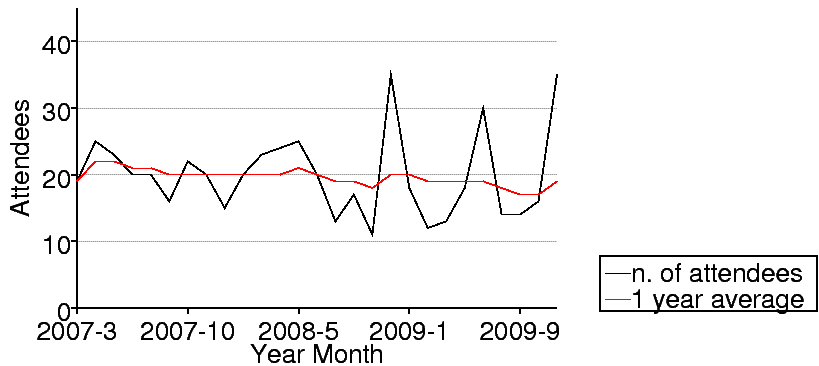
\includegraphics[width=1\hsize]{image200912/kansai.png}
 \end{center}
\caption{$B4X@>$N;22C?M?t?d0\(B}
\label{fig:kansaipeoplechart}
\end{figure}

\begin{table}
\begin{minipage}{0.5\hsize}
 \caption{$B4X@>(BDebian$BJY6/2q;22C?M?t(B(2007$BG/(B)}\label{tab:count2007kansai}
 \begin{center}
  \begin{tabular}{|l|c|p{10em}|}
 \hline
 & $B;22C?M?t(B & $BFbMF(B \\
 \hline
2007$BG/(B3$B7n(B & 19 & $B3+:E$K$"$?$j(B \\
2007$BG/(B4$B7n(B & 25 & goodbye$B!"(Byoutube$B!"%W%m%8%'%/%H%H%i%C%+!<(B\\
2007$BG/(B6$B7n(B & 23 & $B<R2q7@Ls!"%F!<%^!"(Bdebian/rules$B!"(Bbugreport\\
2007$BG/(B7$B7n(B & 20$BA08e(B & OSC-Kansai \\
2007$BG/(B8$B7n(B & 20 & Inkscape$B!"(Bpatch$B!"(Bdpatch\\
2007$BG/(B9$B7n(B & 16 & $B%i%$%V%i%j!"K]Lu!"(Bdebtorrent\\
2007$BG/(B10$B7n(B & 22& $BF|K\8lF~NO!"(BSPAM$B%U%#%k%?(B\\
2007$BG/(B11$B7n(B & 20$BA08e(B & KOF \\   
2007$BG/(B12$B7n(B & 15& $BK:G/2q!"(BiPod touch\\   
 \hline
  \end{tabular}
 \end{center}
\end{minipage}
\begin{minipage}{0.5\hsize}
 \caption{$B4X@>(BDebian$BJY6/2q;22C?M?t(B(2008$BG/(B)}\label{tab:count2008kansai}
 \begin{center}
  \begin{tabular}{|l|c|p{10em}|}
 \hline
 & $B;22C?M?t(B & $BFbMF(B \\
 \hline
2008$BG/(B2$B7n(B & 20 & PC Cluster, GIS, \TeX \\
2008$BG/(B3$B7n(B & 23 & bug report, developer corner, GPG \\
2008$BG/(B4$B7n(B & 24 & coLinux, Debian GNU/kFreeBSD, sid \\
2008$BG/(B5$B7n(B & 25  & ipv6, emacs, ustream.tv\\
2008$BG/(B6$B7n(B & 20  & pbuilder, hotplug, ssl\\
2008$BG/(B8$B7n(B & 13  & coLinux \\
2008$BG/(B9$B7n(B & 17  & debian mentors, ubiquity, DFSG\\
2008$BG/(B10$B7n(B & 11  & cdbs,cdn.debian.or.jp \\
2008$BG/(B11$B7n(B & 35  & KOF \\
2008$BG/(B12$B7n(B & ?  & TeX$B;qNA:n@.%O%s%:%*%s(B\\
 \hline
  \end{tabular}
 \end{center}
\end{minipage}
\begin{minipage}{0.5\hsize}
 \caption{$B4X@>(BDebian$BJY6/2q;22C?M?t(B(2009$BG/(B)}\label{tab:count2009kansai}
 \begin{center}
  \begin{tabular}{|l|c|p{10em}|}
 \hline
 & $B;22C?M?t(B & $BFbMF(B \\
 \hline
2009$BG/(B1$B7n(B & 18 & DMCK, LT \\
2009$BG/(B3$B7n(B & 12 & Git \\
2009$BG/(B4$B7n(B & 13 & Installing sid, Mancoosi, keysign \\
2009$BG/(B6$B7n(B & 18 & Debian Live, bash\\
2009$BG/(B7$B7n(B & 30? & OSC2009Kansai \\
2009$BG/(B8$B7n(B & 14 & DDTSS, lintian \\
2009$BG/(B9$B7n(B & 14 & reportbug, debian mentors\\
2009$BG/(B10$B7n(B & 16 & gdb, packaging \\
2009$BG/(B11$B7n(B & 35 & KOF2009 \\
2009$BG/(B12$B7n(B & ?? & GPS program, OpenStreetMap \\
 \hline
  \end{tabular}
 \end{center}
\end{minipage}
\end{table}

\clearpage

\dancersection{$B:#8e$NM=Dj(B}{Debian JP}

\subsection{$B<!2s$N4X@>(BDebian$BJY6/2q(B}
$B<!2s!"(B2010$BG/(B2$B7n$N4X@>(BDebian$BJY6/2q$O(B 2$B7n(B28$BF|$K(B
$BJ!Eg6hL1%;%s%?!<$G9T$J$$$^$9!#(B

\subsection{$B%*!<%W%s%=!<%9%+%s%U%!%l%s%9(B Kansai @ Kobe 2010}

2010$BG/(B3$B7n(B13$BF|EZMKF|$K(BJR$B?@8M1X$9$0$=$P$N?@8M;T;:6H?66=%;%s%?!<$K$F!"(B
$B%*!<%W%s%=!<%9%+%s%U%!%l%s%9(B Kansai @ Kobe 2010$B$,3+:E$5$l$^$9!#(B
$B4X@>(BDebian$BJY6/2q$G$O!"8=:_;22C$r8!F$$7$F$$$^$9!#(B

% $B:};R$K$9$k$?$a$K!"(B4$B$NG\?t$K$9$kI,MW$,$"$k!#(B
% $B$=$N$?$a$ND4@0(B
\dancersection{$B%a%b(B}{}
\mbox{}\newpage

\printindex
 \cleartooddpage

 \begin{minipage}[b]{0.2\hsize}
  \rotatebox{90}{\fontsize{80}{80} {\gt $B4X@>%G%S%"%sJY6/2q(B} }
 \end{minipage}
 \begin{minipage}[b]{0.8\hsize}

 \vspace*{15cm}
 \rule{\hsize}{1mm}
 \vspace{2mm}
 
\includegraphics[width=2cm]{image200502/openlogo-nd.eps}
 \noindent \Large \bf Debian $BJY6/2q;qNA(B\\ \\
 \noindent \normalfont \debmtgyear{}$BG/(B\debmtgmonth{}$B7n(B\debmtgdate{}$BF|(B \hspace{5mm}  $B=iHGBh(B1$B:~H/9T(B\\
 \noindent \normalfont $B4X@>(B Debian $BJY6/2q(B $B!JJT=8!&0u:~!&H/9T!K(B\\
 \rule{\hsize}{1mm}
 \end{minipage}

\end{document}
